\documentclass[a4paper,11pt]{article}

\title{\textbf{Numerical method for 1D simulation using enthalpy method}}
\author{Joseph Fishlock}

\usepackage{MyStyle}
\usepackage{pdfpages}

\numberwithin{equation}{section}

\begin{document}

\maketitle

\tableofcontents

\clearpage

\section{Non-Dimensional Equations}\label{sec:Non-Dimensional-Equations}

There are two models (non-dimensional systems of conservation equations to be solved).
We work in non-dimensional variables in 1D $(z, \, t)$.
For non-dimensionalisation see~\cpageref{sec:Non-dimensionalisation}.
We use the lagrangian derivative in a moving frame with velocity $V$.

\begin{equation}\label{eq:lagrangian-derivative}
  \frac{Df}{Dt} = \frac{\partial f}{\partial t} + V \frac{\partial f}{\partial z}.
\end{equation}

The three primary non-dimensional variables
bulk enthalpy ($\mathcal{H}_l$),
bulk salinity ($\Theta$ )
and bulk gas ($\Gamma$)
are governed by conservation equations.
All other variables are obtained by an equilibrium enthalpy method calculation.
The liquid Darcy velocity ($W_l$ ) is obtained in the full model by conservation of mass (elliptic pressure equation).
In the reduced model it is free to be imposed as a forcing from a brine convection model.
In both models gas Darcy velocity is calculated as
\begin{equation}\label{eq:Gas-Darcy-Velocity}
W_g = \phi_g V_g = \phi_g \left( \frac{\mathcal{B}}{K(\lambda)} + 2 G(\lambda) \frac{W_l}{\phi_l} \right),
\end{equation}
where $\lambda$ is the ratio of bubble size to tube size.
If we assume a scaling for tube size of the form $R_T = R_0 \phi_l^q$,
then  $\lambda = R_B / R_0 \phi_l^q$.
$K(\lambda)$ and $G(\lambda)$ are empirical functions for a spherical centered bubble in Stokes flow in a cylinder.


\subsection{Full model}\label{sec:Full-model}

We retain the conservation of total volume ($\phi_s + \phi_l + \phi_g = 1$).
This implies changing gas fraction drives liquid flow.
Full model conservation equations

\begin{equation}\label{eq:full-heat}
\frac{D \mathcal{H}}{D t} =
-\frac{\partial}{\partial z} \left[ \mathcal{H}_l W_l \right]
+ \frac{\partial^2 \theta}{\partial z^2},
\end{equation}

\begin{equation}\label{eq:full-salt}
\frac{D \Theta}{D t} =
-\frac{\partial}{\partial z} \left[ W_l (\Theta_l + \mathcal{C}) \right] 
+ \frac{1}{\text{Le}_S} \frac{\partial}{\partial z} \left[ \phi_l \frac{\partial \Theta_l}{\partial z} \right],
\end{equation}

\begin{equation}\label{eq:full-gas}
\frac{D \Gamma}{D t} =
-\frac{\partial}{\partial z} \left[ W_l \chi \omega) \right] 
- \frac{\partial W_g}{\partial z}
+ \frac{\chi}{\text{Le}_\xi} \frac{\partial}{\partial z} \left[ \phi_l \frac{\partial \omega}{\partial z} \right],
\end{equation}

\begin{equation}\label{eq:pressure}
\frac{D \phi_g}{D t} = \frac{\partial}{\partial z} \left[ - \Pi(\phi_l) \frac{\partial p}{\partial z} \right].
\end{equation}

Note: $W_l = -\Pi \frac{\partial p}{\partial z}$.

\subsection{Reduced model}\label{sec:Reduced-model}

We neglect the gas fraction so that $\phi_s + \phi_l = 1$.
The conservation equations remain the same \cref{eq:full-heat,eq:full-salt,eq:full-gas}.
We no longer need to solve for pressure as no flow is driven.
The calculation of the enthalpy method is significantly easier as gas fraction is decoupled from thermal solve.
We can reconstruct approximations to the full phase fractions $\phi^*$ as follows.
In solid region assume $\phi_l^* = \phi_l = 0$, $\phi_g^*=\phi_g$ and $\phi_s^* = 1- \phi_g$.
In other regions  $\phi_s^* = \phi_s$,  $\phi_g^* = \phi_g$ and $\phi_l^* = 1 - \phi_s - \phi_g$.
This means we must impose the extra constraint that prevents more gas accumulating in a region that would already be saturated.
This is done in the numerics by setting  $V_g=0$ if the cell above is such that $\phi_g \ge  1- \phi_s$.

\section{Enthalpy method}\label{sec:Enthalpy-method}
From the primary variables $(\mathcal{H}, \, \Theta, \, \Gamma)$ we seek to reconstruct the other state variables:
temperature ($\theta$ ),
liquid salinity ($\Theta_l$ ),
solid salinity ($\Theta_s$ ),
solid fraction ($\phi_s$ ),
liquid fraction ($\phi_l$ ),
gas fraction ($\phi_g$ ),
and dissolved gas concentration ($\omega$ ).

This is done using the following phase plane information in each region:
\begin{itemize}
\item liquid ($\mathcal{H} >  \mathcal{H}_L$): $\phi_s = 0$ and solid salinity undetermined so set $\Theta_s = -\mathcal{C}$.
\item mush ($\mathcal{H}_E < \mathcal{H} \le  \mathcal{H}_L$): liquidus $\theta = \theta_L(\Theta_l) = - \Theta_l$,
and fresh ice $\Theta_s = - \mathcal{C}$.
\item eutectic ($\mathcal{H}_S < \mathcal{H} \le \mathcal{H}_E$): $\theta = -1$, $\Theta_l = 1$.
\item solid ( $\mathcal{H} \le \mathcal{H}_S$):  $\phi_l=0$, liquid salinity undetermined so set $\Theta_l=1$.
\end{itemize}

The phase boundaries are determined for each region by applying the conditions in both.

The gas saturation state depends on $\Gamma_{\text{sat}} = \chi \phi_l$.

\begin{itemize}
\item Super saturated ($\Gamma  \ge  \Gamma_{\text{sat}}$ ): saturation $\omega=1$ and $\phi_g = \Gamma - \Gamma_{\text{sat}}$.
\item Sub saturated ($\Gamma < \Gamma_{\text{sat}}$ ): $\phi_g=0$ and $\omega = \Gamma / \Gamma_{\text{sat}}$.
\end{itemize}

\subsection{Full enthalpy method}\label{sec:Full-enthalpy-method}
For the full enthalpy method calculation we use the relations:
\begin{equation}\label{eq:full-volume-sum}
\phi_s + \phi_l + \phi_g = 1,
\end{equation}

\begin{equation}\label{eq:full-bulk-enthalpy}
\mathcal{H} = \theta (1 - \phi_g) - \phi_s \text{St},
\end{equation}

enthalpy in each phase is $\mathcal{H}_l = \theta$, $\mathcal{H}_s = \theta - \text{St}$ and $\mathcal{H}_g=0$ 

\begin{equation}\label{eq:full-bulk-salinity}
\Theta = \phi_s \Theta_s + \phi_l \Theta_l - \phi_g \mathcal{C},
\end{equation}

\begin{equation}\label{eq:full-bulk-gas}
\Gamma = \chi \omega \phi_l + \phi_g.
\end{equation}

This is tricky as everything is fully coupled and the enthalpy phase boundaries depend on both salinity and gas content.
See~\cpageref{sec:full-enthalpy-method-derivation} for derivation.

\subsection{Reduced enthalpy method}\label{sec:Reduced-enthalpy-method}
assuming $\phi_s + \phi_l = 1$ for the enthalpy and salt is extremely useful as it reduces to usual enthalpy method~\cite{katz2008}:
\begin{equation}\label{eq:reduced-volume-sum}
\phi_s + \phi_l = 1,
\end{equation}

\begin{equation}\label{eq:reduced-bulk-enthalpy}
\mathcal{H} = \theta - \phi_s \text{St},
\end{equation}

\begin{equation}\label{eq:reduced-bulk-salinity}
\Theta = \phi_s \Theta_s + \phi_l \Theta_l.
\end{equation}

The gas variables can then be solved independent of phase later using only $\Gamma$ and $\phi_l(\mathcal{H}, \, \Theta)$.
This yields the following expressions.

\begin{equation}\label{eq:reduced-liquidus}
\mathcal{H}_L = -\Theta,
\end{equation}

\begin{equation}\label{eq:reduced-eutectic}
\mathcal{H}_E = \frac{\text{St}}{1+\mathcal{C}} (\Theta -1) -1,
\end{equation}

\begin{equation}\label{eq:reduced-solidus}
\mathcal{H}_S = -1 - \text{St}.
\end{equation}

\subsubsection{liquid}\label{ssub:liquid}

\begin{equation*}
\phi_s = 0,
\end{equation*}

\begin{equation*}
\phi_l = 1,
\end{equation*}

\begin{equation*}
\theta = \mathcal{H},
\end{equation*}

\begin{equation*}
\Theta_l = \Theta,
\end{equation*}

\begin{equation*}
\Theta_s = -\mathcal{C}.
\end{equation*}

\subsubsection{mush} \label{ssub:mush}

\begin{equation*}
\phi_l = 1 - \phi_s,
\end{equation*}

\begin{equation*}
\Theta_s = - \mathcal{C},
\end{equation*}

\begin{equation*}
\Theta_l = - \theta,
\end{equation*}

\begin{equation*}
\theta = \mathcal{H} + \phi_s \text{St},
\end{equation*}

\begin{equation*}
\phi_s = \frac{-B - \sqrt{B^2 - 4AC}}{2A},
\end{equation*}

where $A=\text{St}$, $B = \mathcal{H} - \text{St} - \mathcal{C}$, $C = -(\mathcal{H} + \Theta)$.

\subsubsection{eutectic} \label{ssub:eutectic}

\begin{equation*}
\theta = -1,
\end{equation*}

\begin{equation*}
\Theta_l = 1,
\end{equation*}

\begin{equation*}
\phi_l = 1 - \phi_s,
\end{equation*}

\begin{equation*}
\phi_s = \frac{-(1 + \mathcal{H})}{\text{St}},
\end{equation*}

\begin{equation*}
\Theta_s = \frac{\Theta + \phi_s -1}{\phi_s}.
\end{equation*}

Note that this means that on the mush side of the eutectic we get the solid fraction $\phi_s = (1-\Theta) / (1 + \mathcal{C})$.

\subsubsection{solid} \label{ssub:solid}

\begin{equation*}
\phi_l = 0, 
\end{equation*}

\begin{equation*}
\phi_s = 1,
\end{equation*}

\begin{equation*}
\Theta_l = 1,
\end{equation*}

\begin{equation*}
\Theta_s = \Theta,
\end{equation*}

\begin{equation*}
\theta = \mathcal{H} + \text{St}.
\end{equation*}

\section{Spatial discretisation}\label{sec:Spatial-discretisation}

\begin{figure}[h]
  \centering
  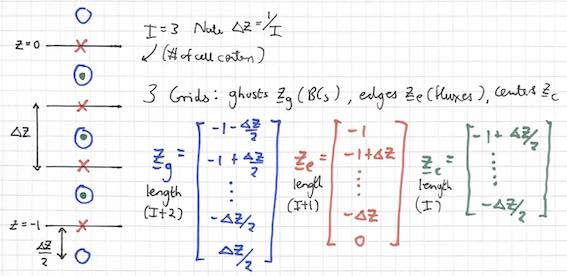
\includegraphics[width=0.8\textwidth]{spatial_discretisation}
  \caption{Diagram of three different girds quantities can sit on in spatial discretisation.}
  \label{fig:spatial_discretisation}
\end{figure}

We discretise the vertical spatial dimension into $I$ cells of width $\Delta z=1 / I$.
Each of these cells has a center and two edges.
The cell centers lie on the centered grid $\boldsymbol{z}_c$.
The cell edges lie on the edge grid $\boldsymbol{z}_e$.
The cell centers plus a ghost cell for boundary conditions at the top and bottom lie on the ghost grid $\boldsymbol{z}_g$.
See~\cref{fig:spatial_discretisation} for a diagram of the grids.


Quantities that lie on the ghost grid are written $\hat{\boldsymbol{f}}=\boldsymbol{f}(\boldsymbol{z}_g, t)$.
Quantities that lie on the edge grid are written $\overline{\boldsymbol{f}}=\boldsymbol{f}(\boldsymbol{z}_e, t)$.
Quantities that lie on the center grid are written $\boldsymbol{f}=\boldsymbol{f}(\boldsymbol{z}_c, t)$.
Note that any quantities on the ghost grid must be given appropriate boundary conditions.


To take derivatives of a quantity on the ghost grid we multiply by the difference matrix $\boldsymbol{D_g}$.
This has dimensions $(I+1, I+2)$ and returns the derivative on the edge grid.
To take derivatives of a quantity on the edge grid we multiply by the difference matrix $\boldsymbol{D_e}$.
This has dimensions $(I, I+1)$ and returns the derivative on the center grid.
Both of these matrices are all zero apart from $-1 / \Delta z$ on the leading diagonal  $(i, \, i)$,
and  $1 / \Delta z$ on the first off diagonal $(i, \, i+1)$.
Note that matrix multiplication is written  $\cdot$ and two quantities on the same grid may be multiplied elementwise.

We introduce two functions for taking ghost grid quantities to edge grid quantities.
First the upwinding function $\mathcal{U}(\text{ghost}, \, \text{edge})$.
This takes a quantity on the ghost grid and a flux on the edge grid and returns their product,
where the ghost value is chosen to be the cell on the side of the edge where the velocity is coming from.
Second the geometric mean function $\mathcal{G}(\text{ghost})$.
This interpolates a quantity on the ghost grid to the edge grid by taking the geometric average of the two neighbouring cell centers.
This is useful as if one of the two cells has no liquid then the edge will have none which makes it impermeable.


We write the spatially discretised equations as

\begin{equation}\label{eq:discretised-enthalpy}
\frac{\partial \mathcal{\boldsymbol{H}}}{\partial t} = -\boldsymbol{D_e} \cdot \overline{\boldsymbol{F}_\mathcal{H}},
\end{equation}

\begin{equation}\label{eq:discretised-salt}
\frac{\partial \boldsymbol{\Theta}}{\partial t} = -\boldsymbol{D_e} \cdot \overline{\boldsymbol{F}_\Theta},
\end{equation}

\begin{equation}\label{eq:discretised-gas}
\frac{\partial \boldsymbol{\Gamma}}{\partial t} = -\boldsymbol{D_e} \cdot \overline{\boldsymbol{F}_\Gamma},
\end{equation}

where the fluxes are given by

\begin{equation}\label{eq:enthalpy-flux}
\overline{\boldsymbol{F}_\mathcal{H}} =
\mathcal{U}(\boldsymbol{\hat{\mathcal{H}}}, \, \overline{\boldsymbol{V}})
+ \mathcal{U}(\hat{\boldsymbol{\mathcal{H}_l}}, \, \overline{\boldsymbol{W_l}})
- \boldsymbol{D_g} \cdot \hat{\boldsymbol{\theta}},
\end{equation}

\begin{equation}\label{eq:salt-flux}
\overline{\boldsymbol{F}_\Theta} =
\mathcal{U}(\boldsymbol{\hat{\Theta}}, \, \overline{\boldsymbol{V}})
+ \mathcal{U}(\hat{\boldsymbol{\Theta_l}} + \mathcal{C}, \, \overline{\boldsymbol{W_l}})
-\frac{1}{\text{Le}_S} \mathcal{G}(\hat{\boldsymbol{\phi}_l}) \boldsymbol{D_g} \cdot \hat{\boldsymbol{\Theta_l}},
\end{equation}

\begin{equation}\label{eq:gas-flux}
\overline{\boldsymbol{F}_\Gamma} =
\mathcal{U}(\boldsymbol{\hat{\Gamma}}, \, \overline{\boldsymbol{V}})
+ \mathcal{U}(\chi \hat{\boldsymbol{\omega}}, \, \overline{\boldsymbol{W_l}})
+ \mathcal{U}(\hat{\boldsymbol{\phi_g}}, \, \overline{\boldsymbol{V_g}})
- \frac{\chi}{\text{Le}_\xi} \mathcal{G}(\hat{\boldsymbol{\phi}_l}) \boldsymbol{D_g} \cdot \hat{\boldsymbol{\omega}}.
\end{equation}

These fluxes give the finite volume first order upwind scheme in space.

The pressure (if used) is given by solving the following linear system

\begin{equation}\label{eq:pressure-solve}
\boldsymbol{M} \cdot \hat{\boldsymbol{p}} = 
\frac{\partial \hat{\boldsymbol{\phi_g}}}{\partial t}
+ \boldsymbol{D_e} \cdot \mathcal{U}(\hat{\boldsymbol{\phi_g}}, \overline{V}),
\end{equation}

where the matrix is given by $\boldsymbol{M} = \boldsymbol{D_e} \cdot \boldsymbol{K} \cdot \boldsymbol{D_g}$.
Where $\boldsymbol{K}$ is the diagonal matrix of size $(I+1, \, I+1)$ formed by $-\overline{\boldsymbol{\Pi}}$.
To prevent the system becoming singular it is necessary to add a small numerical regularisation to this matrix.
This prevents the permeability ever being actually zero.
Boundary conditions are added to the matrix $\boldsymbol{M}$ and forcing term to give
$W_l = 0$ at  $z=0$
and $p=0$ at  $z=-1$.


\section{Solvers}\label{sec:Solvers}

\subsection{lagged solver for full model}\label{sec:lagged-solver-for-full-model}

This solver, chosen as "LU", solves the full model.
You specify a constant timestep.
The pressure equation~\cref{eq:pressure-solve} requires information about the gas fraction at the current and future timestep.
Therefore we take a forward euler timestep of the conservation equations e.g:
\begin{equation}\label{eq:forward-euler}
\boldsymbol{\mathcal{H}}^{n+1} = \boldsymbol{\mathcal{H}}^{n}
- \Delta t \boldsymbol{D}_e \cdot \overline{\boldsymbol{F}_\mathcal{H}}^{n}.
\end{equation}
This step gives a value of the gas fraction at both the current and next timestep which is then used to solve for $W_l$.
In this way the liquid velocity is always lagged one timestep behind the other quantities.

\subsection{Reduced solver forward euler}\label{sec:Reduced-solver-forward-euler}

This solver, chosen as "RED", solves the reduced model using forward euler for a fixed timestep.
It is exactly the same as the lagged solver (see~\cref{sec:lagged-solver-for-full-model}),
but without the extra complication of solving for the liquid velocity and the enthalpy method is much simpler.

\subsection{Scipy solver}\label{sec:Scipy-solver}

This solver, chosen as "SCI", solves the reduced model using the same finite volume upwind scheme.
However, the temporal discretisation is handled entirely by the scipy function solve ivp in the integration module.
This comes with a number of benefits as it handles adaptive timestepping well so long as we specify the max timestep
should be small enough to satisfy the stability of explicit treatment of the thermal diffusion term i.e. $\Delta t < \Delta z^2 / 2$.





\section{Non-dimensionalisation}\label{sec:Non-dimensionalisation}
\includepdf[pages=-]{non-dimensionalisation.pdf}

\section{Full enthalpy method derivation}\label{sec:full-enthalpy-method-derivation}
\includepdf[pages=-]{full_enthalpy_method.pdf}


\bibliographystyle{ieeetr}
\bibliography{/Users/joe/Documents/Citations/My-Library-Project.bib}

\end{document}
